\documentclass[a4paper,10pt]{jsarticle}

% レイアウト
\setlength{\textwidth}{\fullwidth}
\setlength{\textheight}{39\baselineskip}
\addtolength{\textheight}{\topskip}
\setlength{\voffset}{-0.5in}
\setlength{\headsep}{0.3in}
\pagestyle{myheadings}

% パッケージ
\usepackage[dvipdfmx]{graphicx}
\usepackage{amsmath,amssymb,epsfig}
\usepackage{bm}
\usepackage{ascmac}
\usepackage{pifont}
\usepackage{multirow}
\usepackage{enumerate}
\usepackage{cases}
\usepackage{type1cm}
\usepackage{cancel}
\usepackage{url}
\usepackage{listings,jlisting}
% 大きな中括弧
\usepackage{cases}

% 定義
\DeclareMathOperator*{\argmin}{arg\,min}
\DeclareMathOperator*{\argmax}{arg\,max}
\def\vec#1{\mbox{\boldmath$#1$}}
\def\R{{\Bbb R}}

% カウンタの設定
\setcounter{section}{0}
\setcounter{subsection}{0}
\setcounter{subsubsection}{0}
\setcounter{equation}{0}

% キャプションの図をFigに変更
\renewcommand{\figurename}{Fig.}
\renewcommand{\tablename}{Tab.}

% 式番号を式(章番号.番号)に
\makeatletter
\renewcommand{\theequation}{\arabic{section}.\arabic{equation}}
\@addtoreset{equation}{section}
\makeatother

% 表紙
\title{知能システム学特論レポート}
\author{
(DL2班)Caffe on Ubuntu\\
}
\date{2015年\ 6月\ 29日}

% ドキュメントの開始
\begin{document}
\maketitle
\section{報告者}
\begin{list}{}{}
 \item 15344203\hspace{0.5cm} 有田 裕太
 \item 15344206\hspace{0.5cm} 緒形 裕太
 \item 15344209\hspace{0.5cm} 株丹 亮
 \item 12104125\hspace{0.5cm} 宮本 和
\end{list}

\section{進行状況}

\begin{itemize}
\item 理論研究
\item 順伝播型ネットワークについて
\end{itemize}


\section{理論研究}

\subsection{活性化関数}
\subsubsection{単純型細胞と複雑型細胞}


%%%%%%%%%%%%%%%%%%%%%%%%%%%%
単純型細胞と複雑型細胞のモデルをFig.~\ref{fig:単純型細胞と複雑型細胞の
モデル}に示す.(a),(b)は4×4の入力層が中間層のそれぞれと結合していること
を示しており,(c),(d)は入力パターンの位置変化に伴う中間層および出力層の
状態の変化を示している.\\
 中間層は単純型細胞,出力層は複雑型細胞のモデルと
なっており,中間層は位置選択性が厳密であるが,出力層は入力パターンが少し
ずれても活性化する.全体への入力が(c)から(d)のように変化すると,中間層で
も図のように活性化するユニットが変化するが,出力層のユニットは活性化した
ままである.これは出力層は中間層のユニットが一つでも活性化されていれば活
性化するためである.\\
 この2つの細胞をモデル化した二層構造のペアを繰り返す構造が畳み込みニュー
ラルネットに用いられている.物体カテゴリ認識は長年コンピュータには難し
いとされてきたが,近年畳み込みニューラルネットによってそれも解決されつつ
ある.神経科学の分野では,多層の畳み込みニューラルネットが霊長類の脳の高
次視覚野と似た振る舞いを示すことが示されている.

\begin{figure}[t]
 \centering
 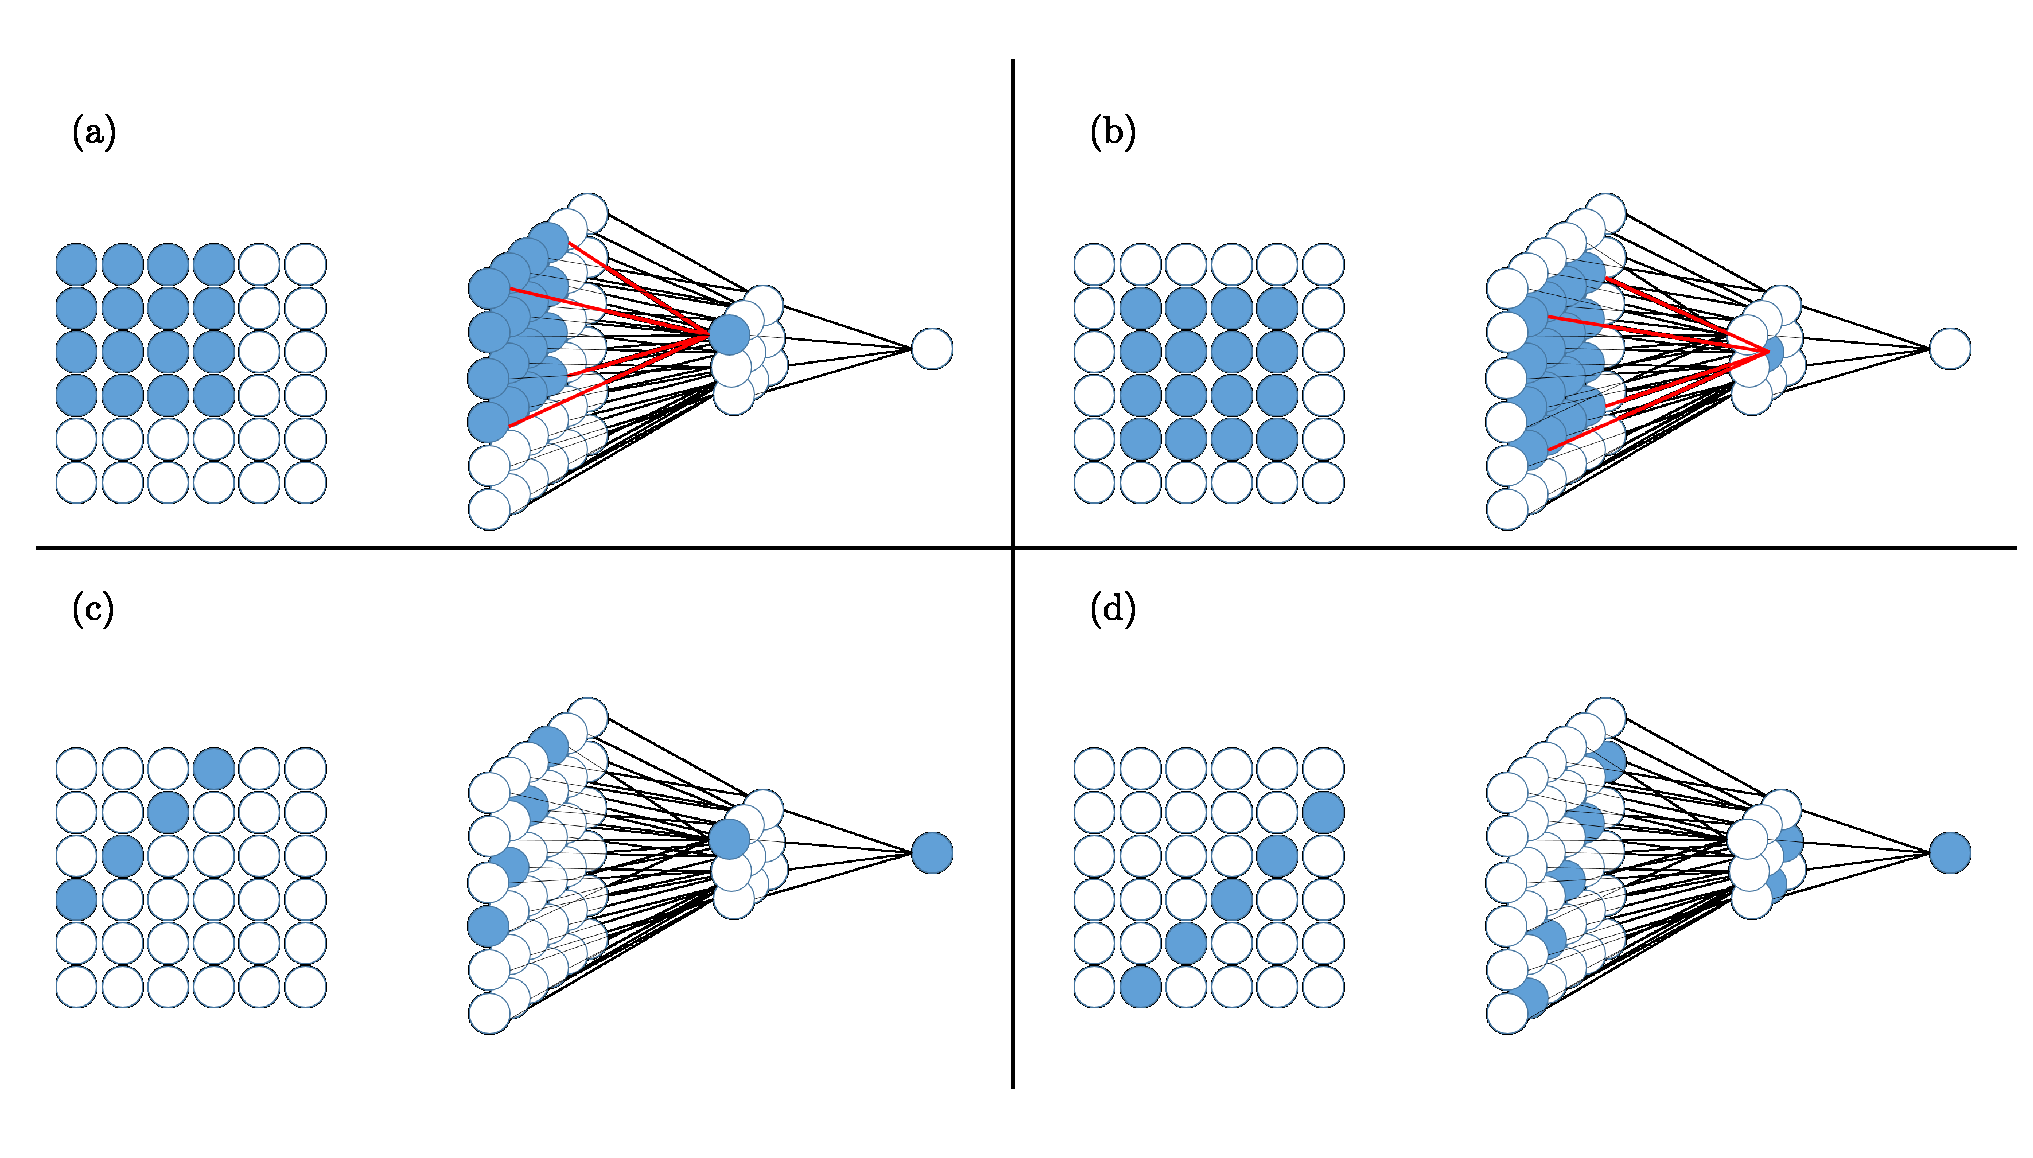
\includegraphics[scale=0.4]{fig/eps/cnn62.eps}
    \caption{単純型細胞と複雑型細胞のモデル}
		\label{fig:単純型細胞と複雑型細胞のモデル}
\end{figure}


\subsection{多層ネットワーク}
Fig.~\ref{fig:2層のネットワーク}に2層構造のネットワークを示す.
Fig.~\ref{fig:2層のネットワーク}~(a)より各層を$l=0,\ 1,\ 2$とすると,$l=1$の層を入力層,$l=2$を中間層,隠れ層,$l=3$を出力層と呼ぶ.
各層のユニットの入出力を区別するために,入力を$\bm{u}^{(l)}$,出力を$\bm{z}^{(l)}$と定義すると,中間層($l=2$)のユニットの出力は以下の式で表される.
\begin{eqnarray}
\label{eq:3a}
  \bm{u}^{(2)} &=& \bm{W}^{(2)}\bm{x} + \bm{b}^{(2)} \\
  \bm{z}^{(2)} &=& \bm{f}(\bm{u}^{(2)})
\end{eqnarray}
$\bm{W}^{(2)}$は入力層と中間層の結合重みであり,$\bm{b}^{(2)}$は中間層のユニットに与えられたバイアスである.
同様にして$\bm{u}^{(3)}$,$\bm{z}^{(3)}$は
\begin{eqnarray}
\label{eq:3b}
  \bm{u}^{(3)} &=& \bm{W}^{(3)}\bm{z}^{(2)} + \bm{b}^{(3)} \\
  \bm{z}^{(3)} &=& \bm{f}(\bm{u}^{(3)})
\end{eqnarray}
となり,任意の階層$L$のネットワークに一般化すると
\begin{eqnarray}
\label{eq:3c}
  \bm{u}^{(l+1)} &=& \bm{W}^{(l+1)}\bm{z}^{(l)} + \bm{b}^{(l+1)} \\
  \bm{z}^{(l+1)} &=& \bm{f}(\bm{u}^{(l+1)})
\end{eqnarray}
と書ける.
$l=1,\ 2,\ 3,\cdots, L-1$の順に繰り返していくと最終的な出力$\bm{y}$を決定することができる.
この出力を決定するのは各層間の結合重み$\bm{W}^{(l)}\ (l=2,\cdots, L)$とユニットのバイアス$\bm{b}^{(l)}\ (l=2,\cdots, L)$である.
これらのパラメータを持つベクトル$\bm{w}$を定義して,$\bm{y}(\bm{x};\bm{w})$と表現する.

% \begin{figure}[tb]
%   \begin{center}
%     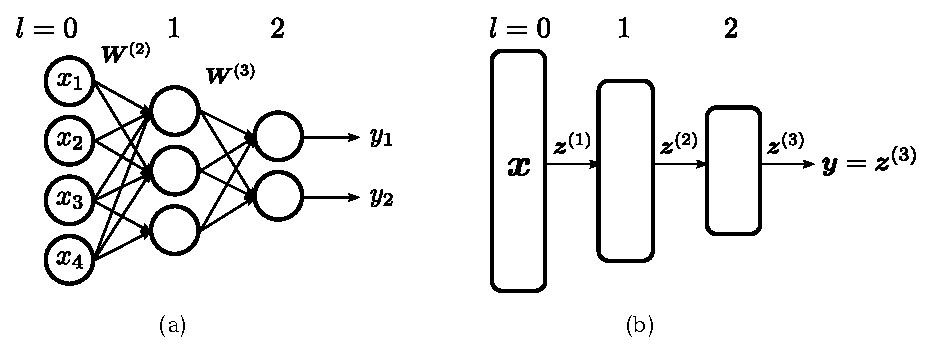
\includegraphics[clip,width=12cm]{fig/eps/unit.eps}
%   \end{center}
%   \caption{2層のネットワーク}
%   \label{fig:2層のネットワーク}
% \end{figure}

\subsection{出力層の設計と誤差関数}
\subsubsection{学習の枠組み}
順伝播型ネットワークが表現する関数$\vec{y}(\vec{x};\vec{w})$をネットワークのパラメータ$\vec{w}$を変えることで変化させ,望みの関数を与えることを考える.
入力$\vec{x}$と望みの出力$\mathrm{d}$のペアを次のように与える.
\begin{eqnarray}
 \{(\vec{x}_{1},\mathrm{d}_{1}),(\vec{x}_{1},\mathrm{d}_{1}),...,(\vec{x}_{N},\mathrm{d}_{N})\}
\end{eqnarray}
これらのペア$(\vec{x},\mathrm{d})$1つ1つを訓練サンプル(training samples)といい,その集合を訓練データ(training data)という.
ネットワーク$\vec{w}$を調整することで訓練データの入出力ペアをできるだけ再現すること学習という.

この場合,ネットワークが表す関数と訓練データとの近さ$(\vec{y}(\vec{x}_{n};\vec{w}))$を誤差関数(error function)で定義する.誤差関数は問題の種別や活性化関数によって異なる.Tab.\ref{000718_27Jun15}に問題の種別ごとの活性化関数と誤差関数の一覧を示す.

% \begin{table}[htb]
% \centering
% \caption{問題の種別ごとの活性化関数と誤差関数}
% \label{000718_27Jun15}
% \begin{tabular}[bt]{|c|c|c|}\hline
%  問題の種別& 出力層の活性化関数&誤差関数 \\ \hline \hline
%  回帰&正接双曲線関数や恒等写像 & 二乗誤差 式\eqref{000645_27Jun15}\\
%  二値分類& ロジスティック関数& 式\eqref{000654_27Jun15}\\
%  多クラス分類& ソフトマックス関数& 交差エントロピー 式\eqref{000700_27Jun15}\\ \hline
% \end{tabular}
% \end{table}

\subsubsection{回帰}
回帰(regression)とは出力連続値をとる関数を対象に訓練データを良く再現する関数を求めることをいう.回帰では活性化関数に正接双曲線関数や恒等写像を用い,評価関数は次式が良く用いられる.
\begin{eqnarray}
 E(\vec{w}) = \displaystyle{\frac{1}{2}}\sum^{N}_{n=1}||\vec{d}_{n}-\vec{y}(\vec{x}_{n};\vec{w})||^{2}\label{000645_27Jun15}
\end{eqnarray}

\subsubsection{二値分類}
二値分類では入力$\vec{x}$に応じて2種類に区別する問題を考える.すなわち,$d\in\{0,1\}$とする.このとき,活性化関数はロジスティック関数$y=1/(1+\exp(-u))$とし,誤差関数は次式で与える.
\begin{eqnarray}
 E(\vec{w})=-\sum^{N}_{n=1}\left[d_{n}\log y(\vec{x}_{n};\vec{w} + (1-d_{n})\log\{1-y(\vec{x}_{n};\vec{w})\})\right]\label{000654_27Jun15}
\end{eqnarray}

\subsubsection{多クラス分類}
多クラス分類とは入力$\vec{x}$に応じて有限個のクラスに分類する問題である.一例としてFig.\ref{010714_27Jun15}に手書き文字認識の例を示す.この問題では活性化関数にはソフトマックス関数(softmax function)が良く用いられる.出力相$l=L$の$k$番目($k=1,...,K$)のユニットの出力は$l=L-1$層の出力を元に次式で与えられ,これをソフトマックス関数という.
\begin{eqnarray}
 y_{k} \equiv z_{k}^{(L)}= \frac{\exp(u_{k}^{(L)})}{\sum^{K}_{j=1}exp(u_{j}^{(L)})}
\end{eqnarray}

また,誤差関数は次式で与える.
\begin{eqnarray}
 E(\vec{w})=-\sum^{N}_{n=1}\sum^{N}_{k=1}d_{nk}\log y_{k}(\vec{x}_{n};\vec{w})\label{000700_27Jun15}
\end{eqnarray}
なお,この関数は交差エントロピー(cross entropy)と呼ばれる.

% \begin{figure}[htbp]
%  	\centering
% 	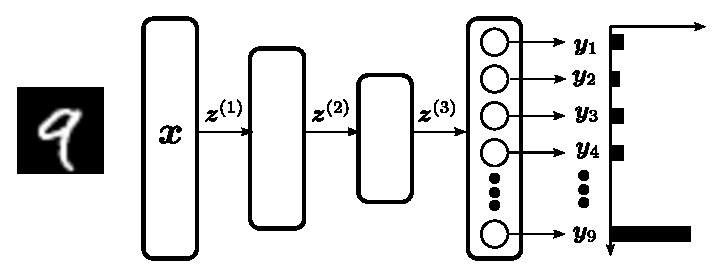
\includegraphics[width=12cm]{./fig/eps/example_digits.eps}
% 	\caption{手書き文字認識の例}
% 	\label{010714_27Jun15}
% \end{figure}

\section{今後の課題}
\begin{itemize}
 \item 理論研究を進める.
 \item Caffeを使いこなす
\end{itemize}

\end{document}